% Здесь пишется содержание второй главы
%
\chapter{\MakeUppercase{Машинное обучение на больших данных}}\label{ch:second}

\vspace{\baselineskip}
В этой главе подробно рассматриваются задачи линейной регрессии и бинарной классификации больших данных.
\vspace{\baselineskip}

\section{Задача регресии}
\subsection{Постановка задачи регрессии}\vspace{\baselineskip}

Постановка задачи линейной регрессии заключается в построении математической модели, которая позволяет предсказывать значение зависимой переменной на основе независимых переменных. Целью является минимизация ошибок и нахождение коэффициентов, которые обеспечивают наиболее точные прогнозы. В данном датасете мы, исходя из разведочного анализа, выяснили предсказываем значение зависимого столбца TOTAL\_FLOOR\_AREA. Также нужно рассчитать оценку качества модели.

Для датасета, заданного представленными колонками, требуется построить модель линейной регрессии для оценки **Площадь квартиры** по всем колличественным и категориальным признакам. 

Для оценки качества обучения следует использовать метрики $RMSE$ и $R^2$.

\vspace{\baselineskip}\subsection{Решение задачи регрессии}\vspace{\baselineskip}

\par Подготовка и кодирование признаков.
\par Для корректной работы трансформеров преобразуем столбцы `HEATING\_COST\_CURRENT`, `HOT\_WATER\_COST\_CURRENT`, `NUMBER\_HABITABLE\_ROOMS`, `NUMBER\_HEATED\_ROOMS` к типу `DoubleType`.
\begin{code}
df = df.withColumn("HEATING_COST_CURRENT", col("HEATING_COST_CURRENT").cast(DoubleType()))
df = df.withColumn("HOT_WATER_COST_CURRENT", col("HOT_WATER_COST_CURRENT").cast(DoubleType()))
df = df.withColumn("NUMBER_HABITABLE_ROOMS", col("NUMBER_HABITABLE_ROOMS").cast(DoubleType()))
df = df.withColumn("NUMBER_HEATED_ROOMS", col("NUMBER_HEATED_ROOMS").cast(DoubleType()))
\end{code}

Отделим от датасета некоторую часть объёмом примерно 1000 строк, и сохраним её на диске как локальный `csv`-файл. Он понадобится в следующей лабораторной работе.
\begin{code}
def save_sample_to_csv(data: DataFrame, file_path: str, 
                       sample_size: int = 1000) -> DataFrame:
\end{code}

Определяем путь для сохранения `csv`-файла.
\begin{code}
path = "/home/user6/Efremenkov_directory/dataset/data/epc_cut_reg.csv"
df = save_sample_to_csv(data=df, file_path=path, sample_size=1000)
\end{code}

Оцениваем, сколько строк в датасете осталось.
\begin{code}
df.count()
\end{code}

Разделим датасет на обучающую и тестовую выборки.
\begin{code}
train_df, test_df = df.randomSplit([0.8, 0.2])
\end{code}

Понятно, что **ключ и адрес** квартиры не оказывает влияния на тип недвижимости. Использовать его в модели нет смысла.
Остальные признаки сгруппируем по их типу:

* **Категориальные** признаки не содержат большого количества категорий, закодируем их `one-hot`-кодировкой.
* **Бинарные** признаки представлены значениями `true` / `false`, которые могут быть интерпретированы как единица и нуль. Поэтому, в кодировании не нуждаются.
* **Количественные** признаки нужно нормализовать / стандартизировать, перед тем, как передавать их в модель.

\begin{code}
categorical_features = [ "PROPERTY_TYPE" ]
numeric_features = [
    "CURRENT_ENERGY_EFFICIENCY", "HEATING_COST_CURRENT", "HOT_WATER_COST_CURRENT", "NUMBER_HABITABLE_ROOMS", "NUMBER_HEATED_ROOMS"
]
\end{code}

Создадим конвейер обработки данных, включающий модель линейной регрессии.
\begin{code}
def create_pipeline(categorical_features: list[str], 
                    numeric_features: list[str], 
                    #binary_features: list[str], binarized_col: str, 
                    #threshold: float, 
                    label_col: str, max_iter: int) -> Pipeline: ... Смотри в приложении...
                    
pipeline = create_pipeline(categorical_features=categorical_features,
                           numeric_features=numeric_features,
                           #binary_features=binary_features,
                           label_col="TOTAL_FLOOR_AREA",
                           max_iter=15)
\end{code}


\par Обучение модели.
Выполним **подбор гиперпараметров** модели линейной регрессии с помощью кросс-валидации на сетке. 
Создаем сетку параметров для кросс-валидации, получив объект `LinearRegression` из конвейера.
Создаем экземпляр `RegressionEvaluator` для оценки модели.
Создаем объект `CrossValidator`.
\begin{code}
param_grid = ParamGridBuilder() \
    .addGrid(pipeline.getStages()[-1].regParam, [0.01, 0.1, 1.0]) \
    .addGrid(pipeline.getStages()[-1].elasticNetParam, [0.0, 0.5, 1.0]) \
    .build()
    
cv_evaluator = RegressionEvaluator(labelCol="TOTAL_FLOOR_AREA",
                                   predictionCol="prediction",
                                   metricName="rmse")
                                   
cross_validator = CrossValidator(estimator=pipeline,
                                 estimatorParamMaps=param_grid,
                                 evaluator=cv_evaluator,
                                 numFolds=5)
\end{code}

Обучаем модель конвейера с использованием кросс-валидации.
\begin{code}
cv_model = cross_validator.fit(train_df)
\end{code}

Выведем параметры **лучшей** модели, определенной в ходе кросс-валидации.
\begin{code}
def get_best_model_params(cv_model: CrossValidatorModel) -> dict[str, float]: ...приложение...
for key, value in get_best_model_params(cv_model=cv_model).items():
    print(f"{key}: {value}")
\end{code}



\vspace{\baselineskip}\subsection{Анализ полученных результатов}\vspace{\baselineskip}

Визуализируем изменение ошибки модели в ходе обучения и рассчитаем метрики на обучающем датасете.
\begin{code}
def plot_training_summary(cv_model: DataFrame) -> None: ... Приложение...
plot_training_summary(cv_model)
\end{code}

\begin{figure}
    \centering
    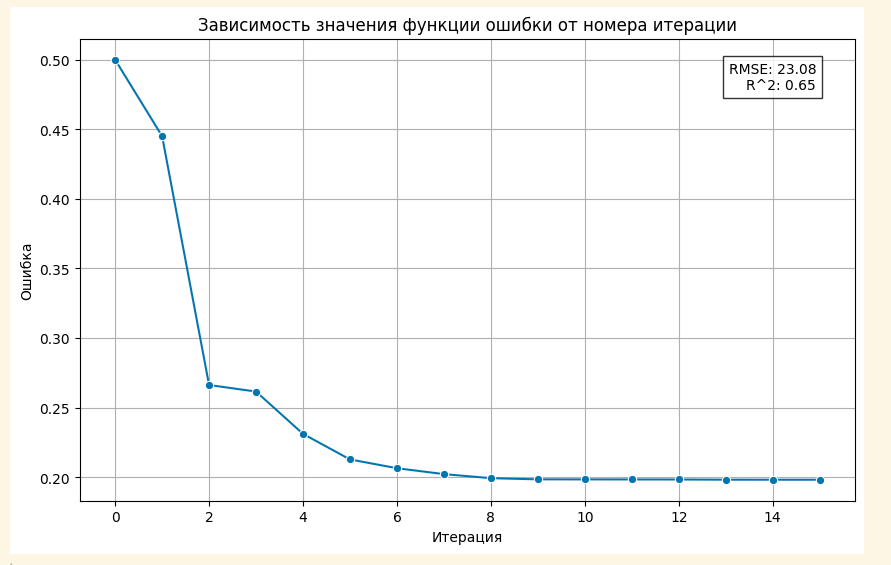
\includegraphics[width=\textwidth]{Content/Images/Zavisimost.png}
    %\caption{Корреляционная матрица датасета}
    \label{fig:ZZFOONI}
\end{figure}

\par Проверка обобщающей способности модели
Выполним предсказания на тестовой выборке. 
Перегруппируем колонки датафрейма, переставив столбец с площадью квартиры в конец, чтобы его значения было удобно сравнивать с предсказанными.
\begin{code}
# Получаем датасет предсказаний
test_df_predictions = cv_model.transform(test_df)

# Извлекаем список колонок, устанавливаем цену на последнее место
right_columns_order = test_df_predictions.columns
right_columns_order.remove("TOTAL_FLOOR_AREA")
right_columns_order.append("TOTAL_FLOOR_AREA")

# Изменяем последовательность колонок и выводим датафрейм
test_df_predictions = test_df_predictions.select(*right_columns_order)
test_df_predictions.show()
\end{code}

Создадим функцию оценки модели: расчета метрик для некоторого датасета, как правило, тестового.
\begin{code}
def evaluate_model(data: DataFrame, metric_name: str) -> float:
\end{code}

Оценим модель на тестовой выборке.
\begin{code}
test_rmse = evaluate_model(test_df_predictions, "rmse")
test_r2 = evaluate_model(test_df_predictions, "r2")

print(f"RMSE on test data: {test_rmse:.2f}")
print(f"R^2 on test data: {test_r2:.2f}")
\end{code}

Результат: 
\begin{enumerate}
\item RMSE on test data: 22.95
\item R\^2 on test data: 0.65
\end{enumerate}
Метрики весьма неплохие для данной модели.

\vspace{\baselineskip}\section{Задача бинарной классификации}

\par В данной части работы рассмотрены:
\begin{itemize}
\item подготовка признаков для рашения задачи **градиентного бустинга** на деревьях решений;
\item создание и обучение модели градиентного бустинга;
\item оценка качества модели.
\end{itemize}

\subsection{Постановка задачи бинарной классификации}\vspace{\baselineskip}

\par Постановка задачи бинарной классификации включает определение, какие данные будут использоваться для обучения модели, выбор метрик для оценки качества модели и определение целевой переменной.

\begin{enumerate}
\item Определение данных

\par Для построения модели необходимо иметь набор данных, который содержит:

\begin{enumerate}
\item Входные признаки (features): Эти данные используются для прогнозирования целевой переменной.
\item Целевая переменная (target variable): Эта переменная представляет собой класс, к которому относится каждый объект в наборе данных. В случае бинарной классификации это обычно два значения, например, 0 и 1.
\end{enumerate}

\item Выбор метрик для оценки качества модели

Для оценки качества модели на этапе тестирования используются различные метрики. Основные метрики в бинарной классификации:

\begin{enumerate}
\item Точность (Precision): Процент объектов, которые действительно принадлежат положительному классу и были корректно определены моделью. [ $Precision = \frac{TP}{TP + FP}$ ] Где ( TP ) — истинные положительные, а ( FP ) — ложные положительные.
\item Полнота (Recall): Процент объектов, которые действительно принадлежат положительному классу и были корректно определены моделью. [ $Recall = \frac{TP}{TP + FN}$ ] Где ( TP ) — истинные положительные, а ( FN ) — ложные отрицательные.
\item F1-мера: Среднее гармоническое точности и полноты. Это метрика, которая учитывает обе ошибки (FP и FN). [ $F1 = 2 \cdot \frac{Precision \cdot Recall}{Precision + Recall}$ ]
\item ROC-AUC (Area Under the Receiver Operating Characteristic Curve): Площадь под кривой ROC, которая показывает, как хорошо модель различает положительные и отрицательные классы при различных порогах вероятности.
\begin{enumerate}
\item Кривая ROC строится на основе значений вероятностей принадлежности положительному классу для всех объектов в наборе данных.
\end{enumerate}

\end{enumerate}

\item Определение целевой переменной
\end{enumerate}
Целевая переменная в бинарной классификации должна быть категориальной и иметь всего два уникальных значения, например, "0" и "1". Значения могут представлять собой различные классы или категории, такие как "заболевал" vs "не заболевал", "покупает" vs "не покупает".

Шаги построения модели
\begin{enumerate}
\item Подготовка данных:
	\begin{enumerate}
	\item Разделить данные на наборы для обучения и тестирования.
	\item Нормализовать или стандартизировать признаки.
	\item Обработать пропущенные значения (например, удалить строки с пропущенными значениями).
	\end{enumerate}
\item Выбор модели:
	\begin{enumerate}
	\item Выбрать подходящую модель бинарной классификации, например, логистическая регрессия, случайный лес или нейронную сеть.
	\end{enumerate}
\item Обучение модели:
	\begin{enumerate}
	\item Обучить модель на наборе данных для обучения.
	\end{enumerate}
\item Оценка качества модели:
	\begin{enumerate}
	\item Оценить качество модели на наборе данных для тестирования.
	\item Использовать выбранные метрики (точность, полнота, F1-мера, ROC-AUC) для оценки производительности модели.
	\end{enumerate}
\item Кросс-валидация:
	\begin{enumerate}
	\item Применить кросс-валидацию для улучшения надежности оценок качества модели.
	\end{enumerate}
\item Оптимизация параметров:
	\begin{enumerate}
	\item Оптимизировать параметры модели с помощью методов, таких как градиентный спуск или случайный поиск.
	\end{enumerate}
\item Интерпретация результатов:
	\begin{enumerate}
	\item Понять, какие признаки влияют на вероятность открытия нового счета.
	\item Делать выводы о том, насколько хорошо модель предсказывает целевую переменную.
	\end{enumerate}
\end{enumerate}

Для датасета, заданного представленными колонками, требуется построить модель градиентного бустинга на деревьях решений для оценки факта того, является ли автомобиль сертифицированным, по всем остальным признакам. 

Для оценки качества обучения следует использовать метрики `Precision` и `Recall`. Оценить максимально возможное значение точности при полноте не менее 60%.

\vspace{\baselineskip}\subsection{Решение задачи бинарной классификации}\vspace{\baselineskip}

\p Для корректной работы трансформеров преобразуем столбцы `HEATING\_COST\_CURRENT`, `HOT\_WATER\_COST\_CURRENT`, `NUMBER\_HABITABLE\_ROOMS`, `NUMBER\_HEATED\_ROOMS` к типу `DoubleType`, а столбец `TOTAL\_FLOOR\_AREA` сделаем бинаризируемым с преобразованием в `Double`

\begin{code}
df = df.withColumn("HEATING_COST_CURRENT", F.col("HEATING_COST_CURRENT").cast(DoubleType()))\n
df = df.withColumn("HOT_WATER_COST_CURRENT", F.col("HOT_WATER_COST_CURRENT").cast(DoubleType()))\n
df = df.withColumn("NUMBER_HABITABLE_ROOMS", F.col("NUMBER_HABITABLE_ROOMS").cast(DoubleType()))\n
df = df.withColumn("NUMBER_HEATED_ROOMS", F.col("NUMBER_HEATED_ROOMS").cast(DoubleType()))\n
\end{code}

\p Бинаризируем столбец TOTAL\_FLOOR\_AREA. Выполняется 1 раз

\begin{code}
udfValueToCategory = udf(valueToCategory, DoubleType())
df = df.withColumn("TOTAL_FLOOR_AREA", udfValueToCategory("TOTAL_FLOOR_AREA") )
\end{code}

\p Выполним **стратифицированное** разделение датасета на обучающую и тестовую выборки.

\begin{code}
def stratified_train_test_split(data: DataFrame, 
                                label_col: str,
                                ratio: float) -> tuple[DataFrame, DataFrame]:
    """
    Разделяет DataFrame на тренировочный и тестовый наборы с учетом стратификации.

    Args:
        data: Исходный DataFrame.
        label_col: Название столбца с меткой.
        ratio: Пропорция разделения данных.

    Returns:
        tuple[DataFrame, DataFrame]: Кортеж из тренировочного и тестового DataFrame.
    """
    # Проверяем корректность доли разделения
    assert (isinstance(ratio, float) and (0.0 <= ratio <= 1.0))
    
    # Формируем разделение для положительных и отрицательных объектов раздельно
    train_df_pos, test_df_pos = (data
                                 .filter(F.col(label_col) == 1)
                                 .randomSplit([ratio, 1 - ratio]))
    train_df_neg, test_df_neg = (data
                                 .filter(F.col(label_col) == 0)
                                 .randomSplit([ratio, 1 - ratio]))
    
    # Объединяем датафреймы
    return (train_df_pos.union(train_df_neg),
            test_df_pos.union(test_df_neg))
\end{code}


\p Выполним балансировку датасета с помощью `oversampling` - подбирает одинаковое количество 1 и 0. 

\begin{code}
def oversample(data: DataFrame, column: str) -> DataFrame:
    """
    Выполняет oversampling положительных классов в DataFrame.

    Args:
        data: Исходный DataFrame.
        column: Название столбца с меткой.

    Returns:
        DataFrame: Датафрейм с выполненным oversampling.
    """
    # Разделим датафрейм на положительные и отрицательные классы
    pos = data.filter(F.col(column) == 1.0)
    neg = data.filter(F.col(column) == 0.0)

    # Получим количество записей в каждом классе
    total_pos = pos.count()
    total_neg = neg.count()
    
    print(total_pos)
    print(total_neg)

    # Если количество положительных классов меньше отрицательных,
    # выполним oversampling
    if total_pos < total_neg:
        # Вычислим количество необходимых дубликатов
        num_duplicates = total_neg - total_pos
        print(num_duplicates)
        # Дублируем положительные записи
        oversampled_pos = pos.withColumn(
            "dummy",
            F.explode(
                F.array_repeat(F.lit(1),
                               num_duplicates // total_pos + 1)
            )
        ).drop("dummy")
        print(num_duplicates // total_pos + 1)
        # Объединим дублированные положительные записи с отрицательными
        balanced_df = neg.union(oversampled_pos)
    else:
        balanced_df = data

    return balanced_df
\end{code}

\p Понятно, что **ключ и адрес** квартиры не оказывает влияния на тип недвижимости. Использовать его в модели нет смысла.

Остальные признаки сгруппируем по их типу:

*\b{Категориальные} признаки не содержат большого количества категорий, закодируем их `one-hot`-кодировкой.
* \b{Бинарные} признаки представлены значениями `true` / `false`, которые могут быть интерпретированы как единица и нуль. Поэтому, в кодировании не нуждаются.
* \b{Количественные} признаки нужно нормализовать / стандартизировать, перед тем, как передавать их в модель.

\begin{code}
categorical_features = [ "PROPERTY_TYPE" ]
numeric_features = [
    "CURRENT_ENERGY_EFFICIENCY", "HEATING_COST_CURRENT", "HOT_WATER_COST_CURRENT", "NUMBER_HABITABLE_ROOMS", "NUMBER_HEATED_ROOMS"
]
\end{code}

\p Обучение модели
Выполним **подбор гиперпараметров** модели линейной регрессии с помощью кросс-валидации на сетке.
Создаем сетку параметров для кросс-валидации, получив объект `GBTClassifier` из конвейера.
Создаем экземпляр `BinaryClassificationEvaluator` для оценки модели.
Создаем объект `CrossValidator`.
Обучаем модель конвейера с использованием кросс-валидации.

\begin{code}
student_hdfs_folder = "Efremenkov_directory"
# Получаем имя пользователя
user_name = os.getenv("USER")

# Путь модели в HDFS
model_hdfs_path = f"hdfs:///user/{user_name}/{student_hdfs_folder}/models/GBT-model"

# Сохраняем модель конвейера в HDFS
try:
    cv_model.bestModel.save(model_hdfs_path)
    print(f"Модель успешно сохранена в \"{model_hdfs_path}\"")
except Exception as e:
    print(f"Ошибка при сохранении модели: {e}")
\end{code}

\p Выведем параметры **лучшей** модели, определенной в ходе кросс-валидации.

\begin{code}
def get_best_model_params(cv_model: CrossValidatorModel) -> dict[str, float]:
    """
    Получает параметры лучшей модели из объекта CrossValidatorModel.

    Args:
        cv_model: Объект CrossValidatorModel, содержащий лучшую модель.

    Returns:
        Dict[str, float]: Параметры лучшей модели.
    """
    best_model = cv_model.bestModel
    best_params = {
        "maxDepth": best_model.stages[-1].getMaxDepth(),
        "stepSize": best_model.stages[-1].getStepSize(),
        "maxIter": best_model.stages[-1].getMaxIter()
    }
    return best_params
\end{code}

\begin{code}
for key, value in get_best_model_params(cv_model=cv_model).items():
    print(f"{key}: {value}")
\end{code}

Результат:
\begin{enumerate}
\item maxDepth: 5
\item stepSize: 0.01
\item maxIter: 30
\end{enumerate}

\p Анализ обученной модели
\p Рассчитаем метрики на тестовом датасете.

\begin{code}
# Получаем датасет предсказаний
test_df_predictions = cv_model.transform(test_df)

# Извлекаем список колонок, устанавливаем цену на последнее место
right_columns_order = test_df_predictions.columns
right_columns_order.remove("TOTAL_FLOOR_AREA")
right_columns_order.append("TOTAL_FLOOR_AREA")

# Изменяем последовательность колонок и выводим датафрейм
test_df_predictions = test_df_predictions.select(*right_columns_order)
\end{code}

\begin{code}
def evaluate_model(data: DataFrame, 
                   label_col: str) -> dict[str, float]:
    """
    Оценивает модель с использованием метрик точности, полноты и F1-score.

    Args:
        data: DataFrame, содержащий предсказания и фактические метки.
        label_col: Название колонки с меткой.

    Returns:
        dict[str, float]: Словарь с метриками точности, полноты и F1-score.
    """
    # Вычисляем TP, FP, FN
    tp = data.filter((F.col(label_col) == 1) &
                     (F.col("prediction") == 1)).count()
    fp = data.filter((F.col(label_col) == 0) &
                     (F.col("prediction") == 1)).count()
    fn = data.filter((F.col(label_col) == 1) &
                     (F.col("prediction") == 0)).count()

    # Вычисляем метрики
    precision = tp / (tp + fp) if (tp + fp) > 0 else 0
    recall = tp / (tp + fn) if (tp + fn) > 0 else 0
    f1 = (2 * (precision * recall) / (precision + recall)
        if (precision + recall) > 0 else 0)

    # Возвращаем словарь с метриками
    return {
        "precision": precision,
        "recall": recall,
        "f1": f1
    }
\end{code}

\begin{code}
metrics = evaluate_model(test_df_predictions, "TOTAL_FLOOR_AREA")
print(f"Metrics: {metrics}")
\end{code}

\p Результат Metrics: 
\begin{enumerate}
\item 'precision': 0.859179580674567 
\item 'recall': 0.7177807853154796 
\item 'f1': 0.7821408926234328
\end{enumerate}

\p Наблюдаем довольно высокую точность при высокой полноте. Попробуем подобрать `threshold`, чтобы максимизировать точность, но при этом удерживать полноту на заданном в постановке задачи уровне.
Сначала рассчитаем `AUC ROC`, визуализируем `ROC` и `PR`-кривые и оценим ситуацию.

\begin{figure}
    \centering
    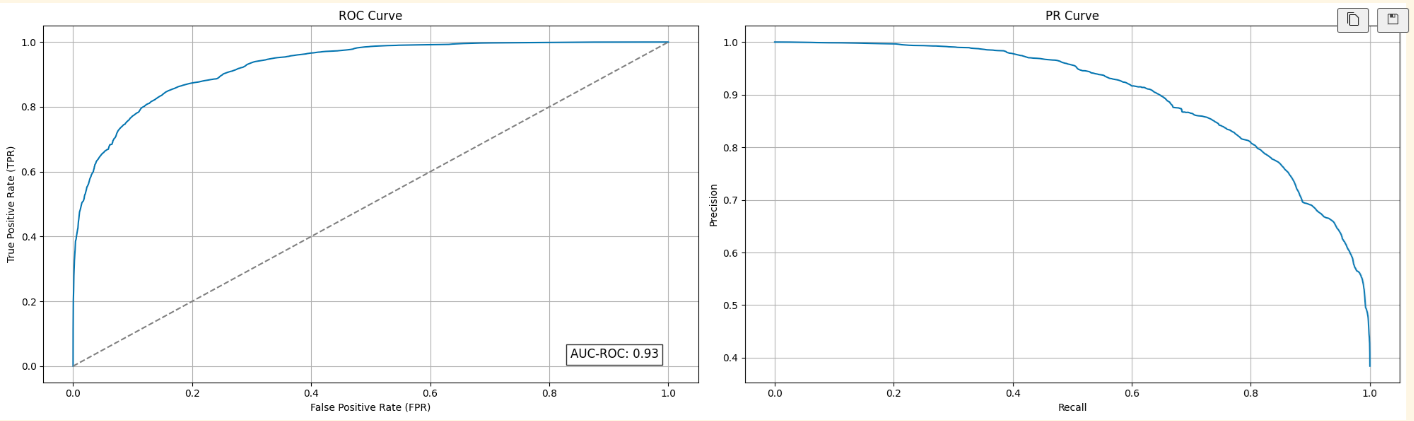
\includegraphics[width=\textwidth]{Content/Images/AUC_ROC.png}
    %\caption{Корреляционная матрица датасета}
    \label{fig:ZZFOONI}
\end{figure}

\vspace{\baselineskip}\subsection{Анализ полученных результатов}\vspace{\baselineskip}

\par Определим вероятность -- границу разделения, при которой `Recall` не меньше 60\%.
\begin{code}
threshold_probability = pd_dataframe[pd_dataframe['TPR'] >= 0.60]['probability'].max()
print(f"Вероятность -- граница разделения, при которой TPR не меньше 60\%: {threshold_probability:.2f}")
\end{code}
Вероятность -- граница разделения, при которой TPR не меньше 60\%: 0.70

\par Рассчитаем метрики на тестовом датасете повторно, с учетом вычисленного `threshold` для вероятности.
\begin{code}
cv_model.bestModel.stages[-1].setThresholds([1 - threshold_probability, 
                                             threshold_probability])
test_df_predictions = cv_model.transform(test_df)
metrics = evaluate_model(test_df_predictions, "TOTAL_FLOOR_AREA")
print(f"Metrics: {metrics}")
\end{code}
Результат Metrics: 
\begin{enumerate}
\item 'precision': 0.9164163632014035, 
\item 'recall': 0.6001314226281914, 
\item 'f1': 0.7252923526797572}
\end{enumerate}

\vspace{\baselineskip}\section{Выводы}\vspace{\baselineskip}

\par Обученная модель обладает очень хорошим качеством и не требует его дальнейшего улучшения.
